\documentclass[notitlepage]{article}

\usepackage[left=1in, right=1in, top=1in, bottom=1in]{geometry}
\usepackage[english]{babel}
\usepackage{titling}
\usepackage{float}
\usepackage{subfig}
\usepackage{graphicx}
\usepackage{varwidth}
\usepackage{hyperref}
 
\graphicspath{{Main_Images/}}

\pretitle{\begin{center}\Huge\bfseries}
\posttitle{\par\end{center}\vskip 0.5em}
\preauthor{\begin{center}\Large\ttfamily}
\postauthor{\end{center}}
\predate{\par\large\centering}
\postdate{\par}

\title{C.LABEL-VR Handout}
\date{\today}
\begin{document}

\maketitle
%\thispagestyle{empty}

%\qquad


\bigskip
\bigskip
\bigskip
\section{UI-Interaction}
\begin{figure}[H]
   \centering
    \subfloat[]{{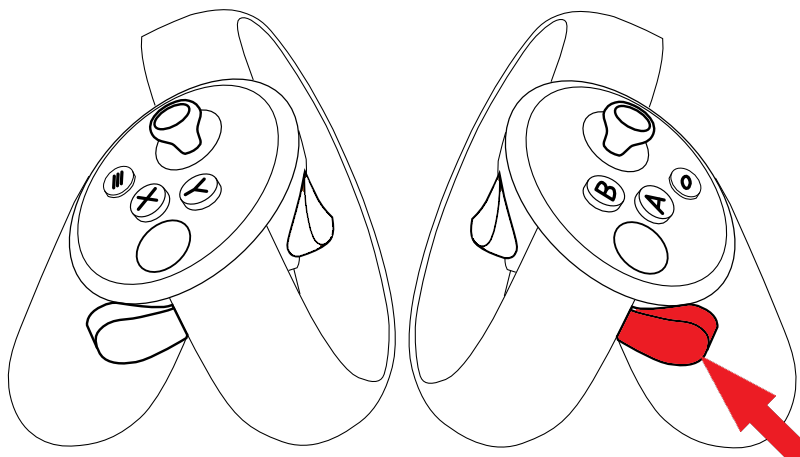
\includegraphics[width=7cm]{Controllers_rightgrip}\label{fig:RightGrip1}}}%
    \quad
    \subfloat[]{{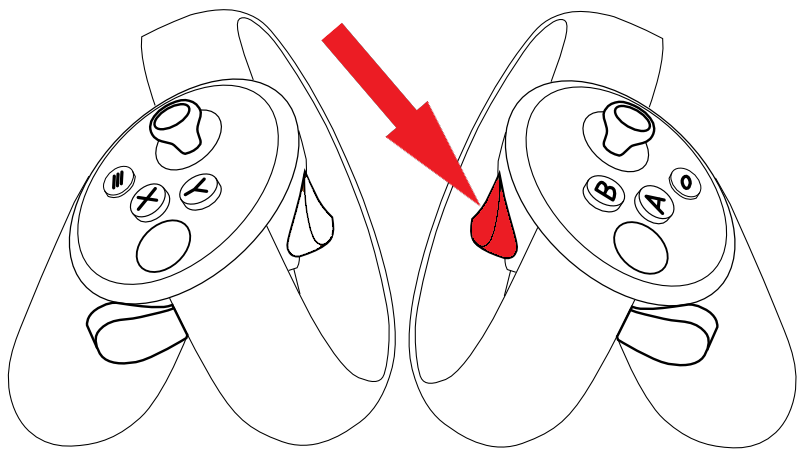
\includegraphics[width=7cm]{Controllers_righttrigger}\label{fig:RightTrigger1}}}%
    \caption{UI-Interaction Controls}\label{fig:UI-Interaction}%
\end{figure}

\qquad
\begin{enumerate}
\item Press the right Grip Button (Figure \ref{fig:RightGrip1}) \\
\item Aim at desired UI-Element (Button, Inputfield, ...)\\
\item Click on this UI-Element with the right Trigger Button (Figure \ref{fig:RightTrigger1})
\end{enumerate} 


%----------------------------------------------------------------------------------------------------------

\section{Navigation}
\begin{figure}[H]
   \centering
	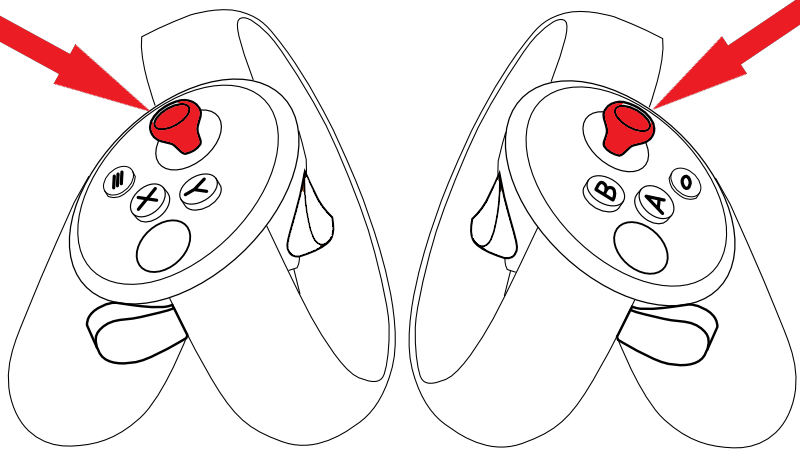
\includegraphics[width=11cm]{Controllers_sticks}%
    \caption{Navigation Controls}\label{fig:LeftRightSticks}%
\end{figure}

\begin{center}
\begin{varwidth}[t]{.5\textwidth}
Left Controller:
\begin{itemize}
\item \textbf{Left}: Move to \textbf{left}
\item \textbf{Right}: Move to \textbf{right}
\item \textbf{Up}: Move to \textbf{front}
\item \textbf{Down}: Move to \textbf{back}
\end{itemize}
\end{varwidth}% <---- Don't forget this %
\hspace{4em}% <---- Don't forget this %
\begin{varwidth}[t]{.5\textwidth}
Right Controller:
\begin{itemize}
\item \textbf{Left}: Turn to \textbf{left}
\item \textbf{Right}: Turn to \textbf{right}
\item \textbf{Up}: Move \textbf{up}
\item \textbf{Down}: Move \textbf{down}
\end{itemize}
\end{varwidth}
\end{center}

\qquad
\subsection{Free Fly Mode}

Use the controls from above to navigate with a constant movement based on acceleration and deceleration.

\qquad
\subsection{Teleport Mode}

Use the controls from above to navigate with quick position shifts on every control input.

\newpage
\subsubsection{Pointer-Teleport}

\begin{figure}[H]
   \centering
    \subfloat[]{{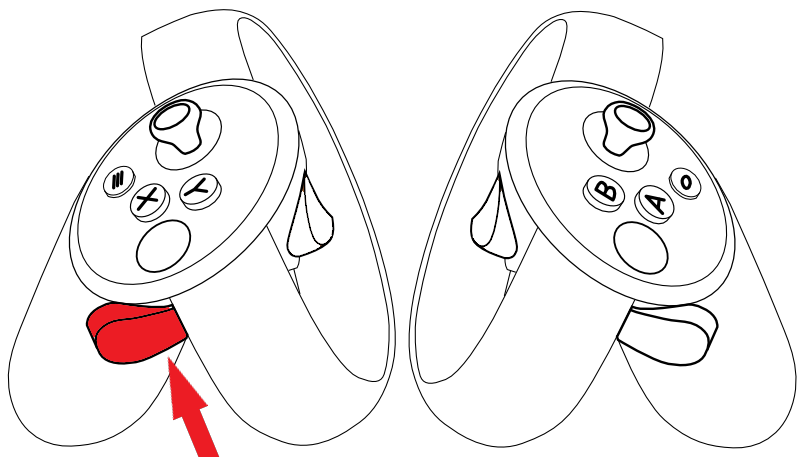
\includegraphics[width=5cm]{Controllers_leftgrip}\label{fig:Controllers_leftgrip}}}%
    \quad
    \subfloat[]{{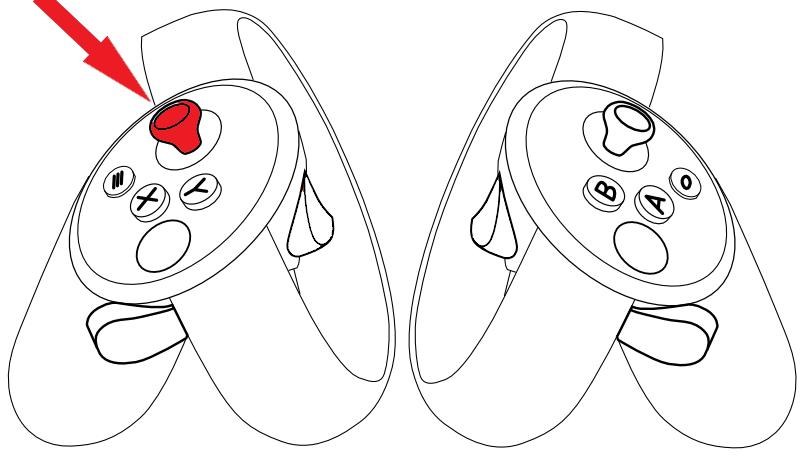
\includegraphics[width=5cm]{Controllers_leftStick}\label{fig:Controllers_leftStick}}}%
    \quad
    \subfloat[]{{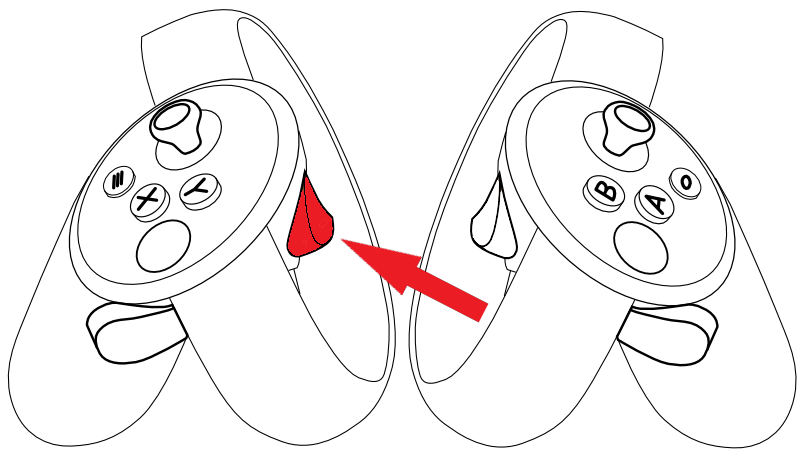
\includegraphics[width=5cm]{Controllers_leftTrigger}\label{fig:Controllers_leftTrigger}}}%
    \caption{Pointer Teleport Controls}\label{fig:UI-Interaction}%
\end{figure}

\begin{enumerate}
\item Press the left Grip Button (Figure \ref{fig:Controllers_leftgrip}) \\
\item Change the lenght of the pointer by pushing the left stick up or down (Figure \ref{fig:Controllers_leftStick})\\
\item Press the left Trigger Button to teleport to the end of the pointer (Figure \ref{fig:Controllers_leftTrigger})
\end{enumerate} 

%----------------------------------------------------------------------------------------------------------

\bigskip
\bigskip
\bigskip
\section{Annotation}

\subsection{Choose Label Class}

\subsubsection{Zapping}

\begin{figure}[H]
   \centering
	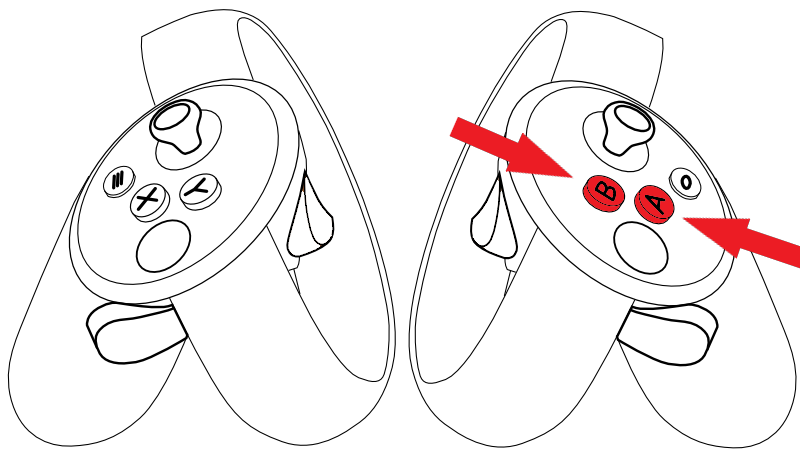
\includegraphics[width=10cm]{Controllers_A&B}%
    \caption{Zapping through Label Classes}\label{fig:Controllers_A&B}%
\end{figure}

\qquad
Zapp through the label classes by pressing the A or the B Button on your right Controller.

\subsubsection{Pipette}

\begin{figure}[H]
   \centering
    \subfloat[]{{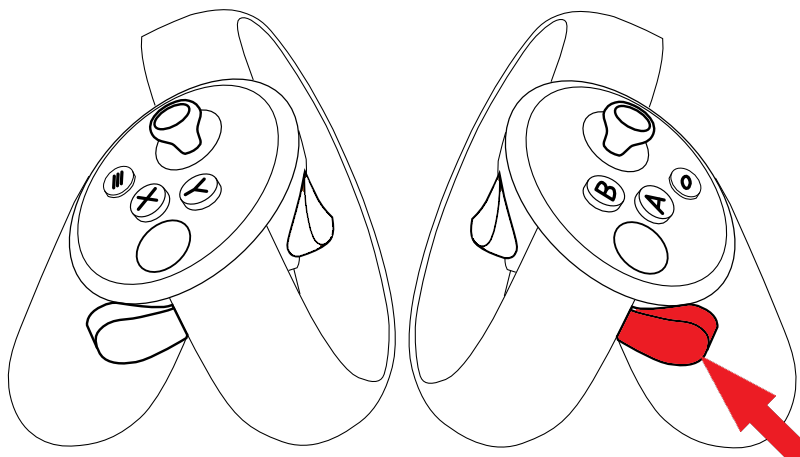
\includegraphics[width=7cm]{Controllers_rightgrip}\label{fig:Controllers_rightgrip}}}%
    \quad
    \subfloat[]{{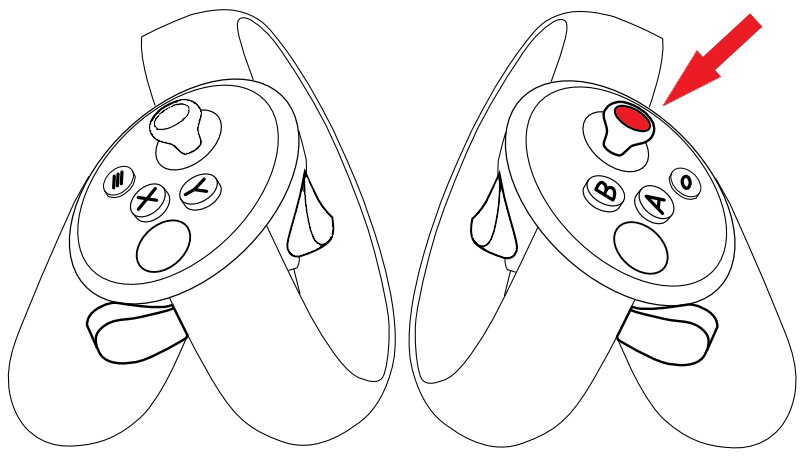
\includegraphics[width=7cm]{Controllers_RightStickPress}\label{fig:Controllers_RightStickPress}}}%
    \caption{Getting Label Class through Pipette}\label{fig:UI-Interaction}%
\end{figure}

\qquad
\begin{enumerate}
\item Press the right Grip Button (Figure \ref{fig:Controllers_rightgrip}) \\
\item Aim at a point which has the label you want to choose\\
\item Click onto the right stick to get the label class from this point (Figure \ref{fig:Controllers_RightStickPress})
\end{enumerate} 

\bigskip
\bigskip
\bigskip
\subsection{Pointer Annotation}

\begin{figure}[H]
   \centering
    \subfloat[]{{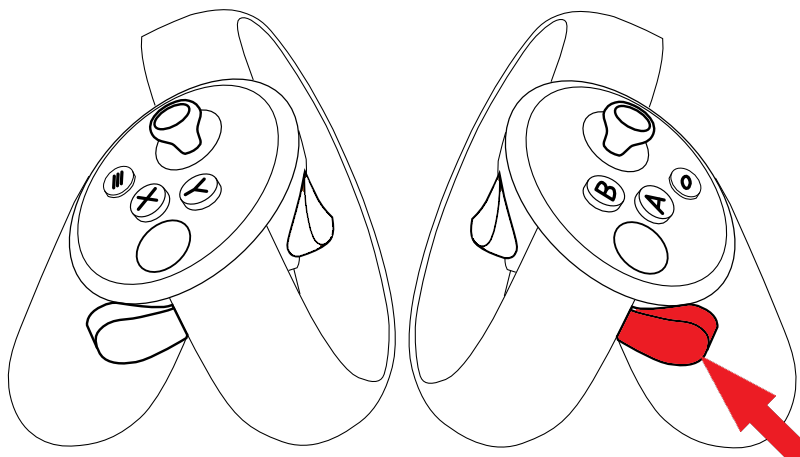
\includegraphics[width=7cm]{Controllers_rightgrip}\label{fig:RightGrip2}}}%
    \quad
    \subfloat[]{{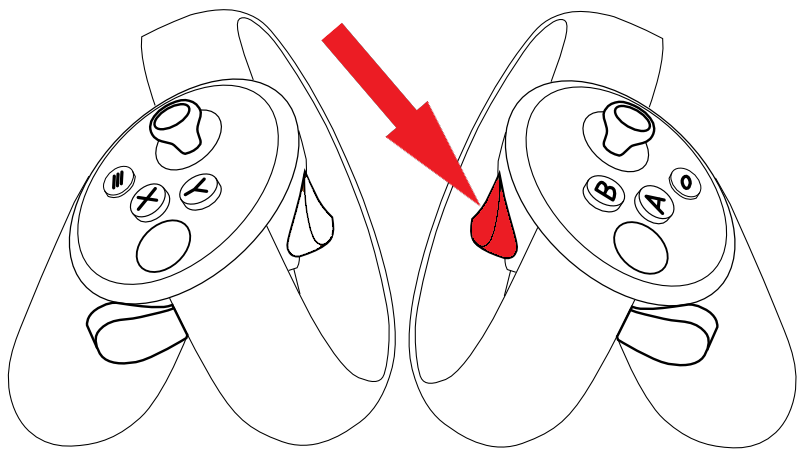
\includegraphics[width=7cm]{Controllers_righttrigger}\label{fig:RightTrigger2}}}%
    \caption{Pointer Annotation Controls}\label{fig:UI-Interaction}%
\end{figure}

\qquad
\begin{enumerate}
\item Press the right Grip Button (Figure \ref{fig:RightGrip2}) \\
\item Aim at desired point you want to annotate\\
\item Click on this Point with the right Trigger Button (Figure \ref{fig:RightTrigger2})
\end{enumerate} 

\subsection{Touch Annotation}

\begin{figure}[H]
   \centering
	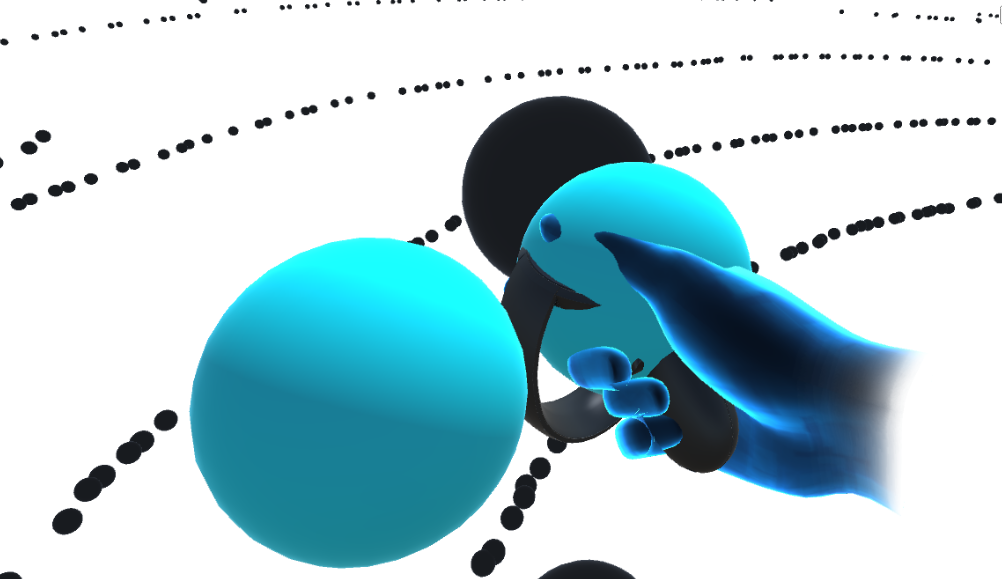
\includegraphics[width=10cm]{TouchLabeling}%
    \caption{Touch Annotation}\label{fig:TouchAnnotation}%
\end{figure}

\qquad
\begin{enumerate}
\item Navigate near to a desired Point \\
\item Move your hand towards the desired point like in Figure \ref{fig:TouchAnnotation}\\
\item If you reach the Point with your hand it should be annotated and you should get a vibration feedback
\end{enumerate} 

\bigskip
\bigskip
\bigskip
\subsection{Cluster Annotation}

\begin{figure}[H]
   \centering
    \subfloat[]{{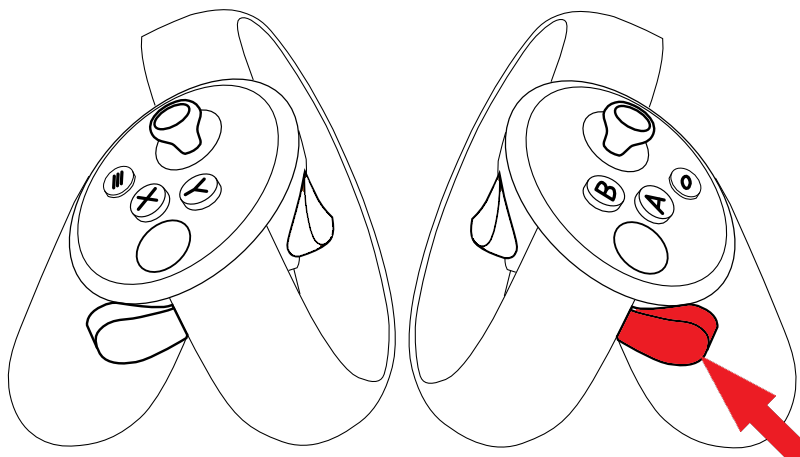
\includegraphics[width=5cm]{Controllers_rightgrip}\label{fig:RightGrip3}}}%
    \quad
    \subfloat[]{{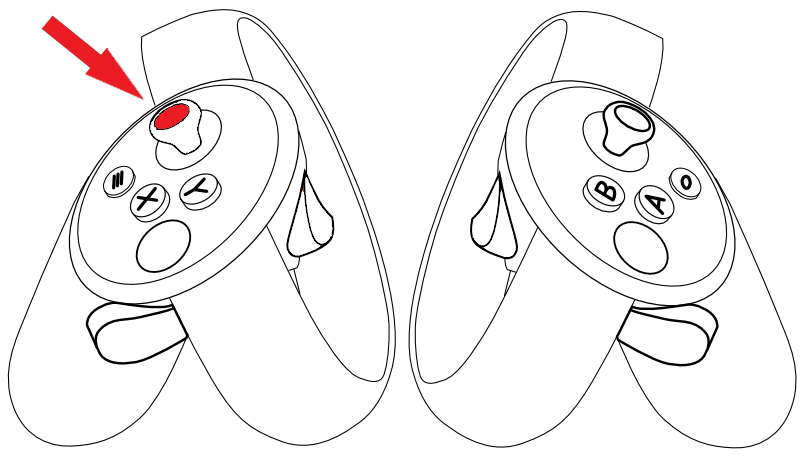
\includegraphics[width=5cm]{Controllers_LeftStickPress}\label{fig:Controllers_LeftStickPress}}}%
    \quad
    \subfloat[]{{\includegraphics[width=5cm]{Controllers_rightTrigger}\label{fig:RightTrigger3}}}%
    \caption{Cluster Annotation Controls}\label{fig:UI-Interaction}%
\end{figure}

\qquad
\begin{enumerate}
\item Press the right Grip Button (Figure \ref{fig:RightGrip3}) \\
\item Aim at desired Point you want and press and hold the left stick (Figure \ref{fig:Controllers_LeftStickPress})\\
\item Click on this Point with the right Trigger Button (Figure \ref{fig:RightTrigger3})
\end{enumerate}  

%----------------------------------------------------------------------------------------------------------
\section{Application Menu}

\begin{figure}[H]
   \centering
    \subfloat[]{{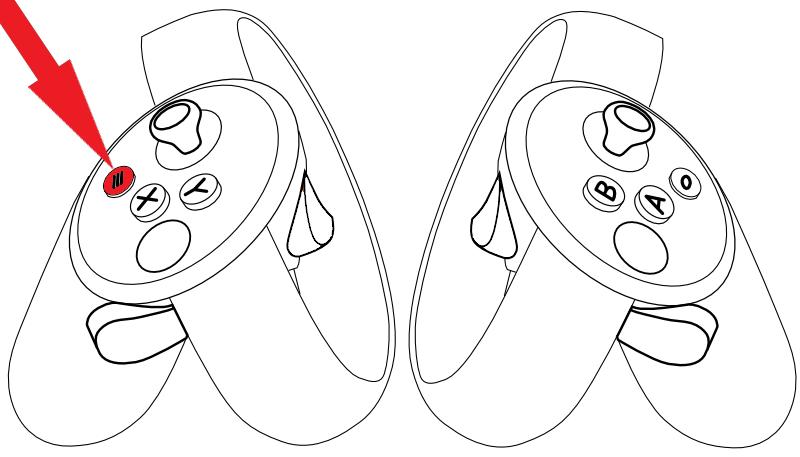
\includegraphics[width=6cm]{Controllers_options}\label{fig:Controllers_options}}}%
    \quad
    \subfloat[]{{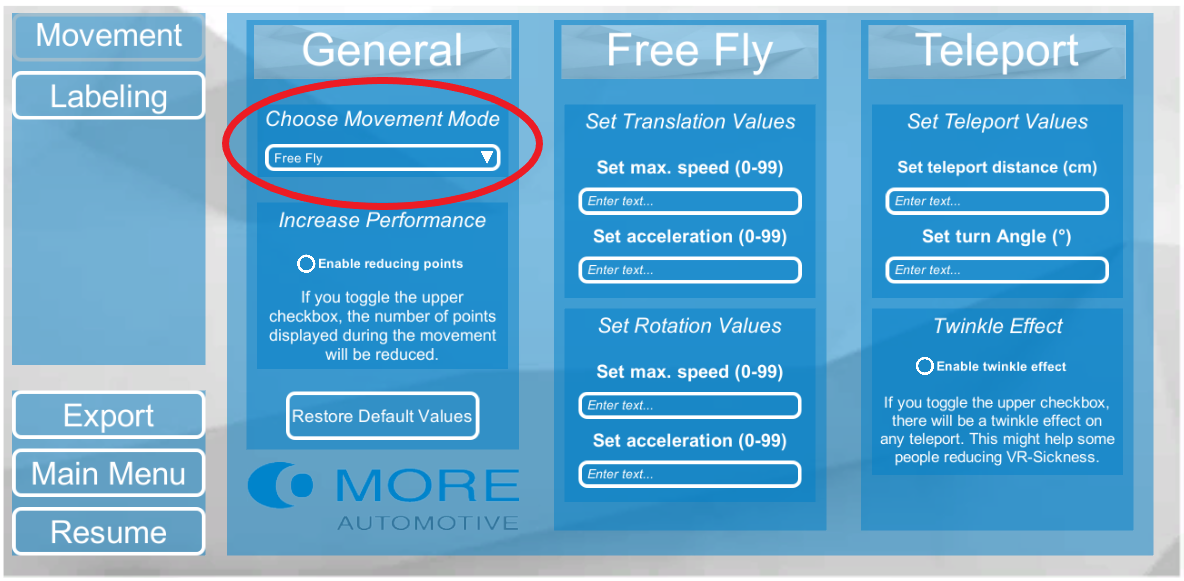
\includegraphics[width=9cm]{InGameMenu}\label{fig:InGameMenu}}}%
    \caption{Opening of the Application Menu}\label{fig:UI-Interaction}%
\end{figure}

\qquad
\begin{enumerate}
\item Press the Option Button on the left controller (Figure \ref{fig:Controllers_options}) \\
\item Do the desired option changes, for example change the movement mode (red circle in Figure \ref{fig:InGameMenu})\\
\item Click on Resume to close the Application
\end{enumerate}  


\end{document}